\section{Explore Phase: Estimating the Scene Geometry and Free Space}
\label{sec:free_space}

In this section, we describe our high-level strategy for data acquisition, as well as our multi-view stereo processing pipeline for estimating the scene geometry and free space.
Our goals in this section are twofold.
First, we would like to obtain a rough estimate of the scene geometry, in the form of a triangle mesh in real-world coordinates.
Second, we would like to obtain a strictly conservative estimate of the free space, in the form of an occupancy volume in real-world coordinates.
Together, these complimentary scene representations will enable us to plan trajectories that maximize the quality of a 3D reconstruction.

\vspace{-12pt}
\paragraph{Drone Camera Hardware}
Our system requires access to a drone camera that can be commanded to fly along pre-specified camera trajectories, given in GPS coordinates (i.e., latitude, longitude, altitude).
The drone camera must also take geotagged images of the scene at roughly constant intervals (e.g., one image every few meters).
We require geotagged images, in order to establish a correspondence between the physical world and the arbitrary coordinate system of our multi-view stereo reconstruction.
In our system, we use the 3D Robotics Solo drone \cite{3dr:2017b} equipped with a GoPro Hero 4 camera.

\vspace{-12pt}
\paragraph{User Input}
Our system requires two bounding boxes as input, each of which can easily be drawn by a user on a 2D map (e.g., Google Maps) and extruded vertically.
The first bounding box, $\mathbf{b}_s$, specifies the volume that the user wants to scan.
The second bounding box, $\mathbf{b}_c$, specifies the volume that the drone is allowed to fly within.
We require that $\mathbf{b}_c$ be made sufficiently tall, so that the entire ceiling of $\mathbf{b}_c$ is free of obstacles.
This requirement is necessary to give our drone some non-trivial region of free space that it can safely explore, prior to resolving any scene geometry.
We do not assume initially that any other space is free.

\vspace{-12pt}
\paragraph{Initial Camera Trajectory}
Our system begins by flying the drone in an elliptical orbit trajectory around the ceiling of $\mathbf{b}_c$, pointing the camera at the center of $\mathbf{b}_s$.
For the scenes we consider in this paper, this initial elliptical trajectory consumes roughly 25\% of our drone's travel budget.

\vspace{-12pt}
\paragraph{Dense Multi-View Stereo}
After we have flown an initial camera trajectory, the first step in our image processing pipeline is to run the structure-from-motion software VisualSFM \cite{wu:2013,wu:2007,wu:2011b,wu:2011a} on the sequence of images acquired by our drone.
Our next step is to run the depth map reconstruction step of the Multi-View Environment (MVE) \cite{fuhrmann:2015}.
In our implementation, we set the \emph{scale} parameter of MVE such that the reconstructed depth maps will be at a resolution of at least 512$\times$512 (e.g., if the images we originally capture are 2048$\times$2048, we set the \emph{scale} parameter to 2).
For the scenes we consider in this paper, computing structure-from-motion and dense multi-view stereo takes roughly 15 minutes, and is the dominant cost in our explore phase.

\vspace{-12pt}
\paragraph{Mapping Between Coordinate Systems}
We perform all our trajectory planning in real-world coordinates, using the UTM coordinate system \cite{usgs:2001}.
UTM coordinates are similar to GPS coordinates, in the sense that they describe positions on the surface of the Earth.
However, unlike GPS coordinates, the UTM coordinate axes are approximately orthogonal, and the default UTM units are meters.
Together, these properties make UTM coordinates well-suited for trajectory planning.

%However, it is convenient for a user to specify input bounding boxes in GPS coordinates (e.g., by drawing on a 2D map).
%Moreover, the communication interface to our drone requires that we specify trajectories in GPS coordinates.
%We use the utm Python library [???] to map back and forth between GPS and UTM coordinates.

In order to use our reconstructed scene geometry for trajectory planning, we must establish a correspondence between the UTM coordinate system and the arbitrary coordinate system of the reconstructed geometry.
We estimate this correspondence by considering our sequence of geotagged camera positions (in UTM coordinates), and the sequence of estimated camera positions recovered during our structure-from-motion step (in reconstruction coordinates).
We estimate the similarity transform that maps from reconstruction coordinates to UTM coordinates using standard numerical techniques \cite{sorkine:2017}.

\vspace{-12pt}
\paragraph{Obtaining an Oriented Point Cloud and Occupancy Volume}
We generate an oriented point cloud of the scene geometry, and an occupancy volume of the scene's free space, using our own modified version of MVE.
Given a collection of camera poses and corresponding depth images, we obtain our point cloud by projecting each depth image into reconstruction coordinates, and then into UTM coordinates.

We generate an occupancy volume of the free, occupied, and unknown space using a simple space carving algorithm.
For every depth observation in every depth image, we project the depth observation and corresponding camera into UTM coordinates.
This projection defines a ray that starts at the camera and ends at the depth observation.
In our occupancy volume, we mark every interior voxel along this ray as being free, and we mark the last voxel along this ray as being occupied.
After having generated our occupancy volume in this way, we create an extra safety buffer around obstacles by dilating the occupied space by 4 meters in every direction.
This safety buffer is conservative, in the sense that it is roughly twice the diameter of the largest localization errors we observed on our drone hardware during field testing.
We consider all unmarked voxels to be unknown.
We store our occupancy volume efficiently in an OctoMap data structure \cite{hornung:2013}.

After this space carving step is complete, we assume that our occupancy volume strictly underestimates the free space in the scene.
This assumption is justified by the following three observations.
First, MVE\ aggressively filters outlier depth observations. So, although MVE does not produce a depth observation at every pixel of every depth image, the observations that MVE does produce tend to be very reliable.
Second, we only mark a voxel as being free if there is explicit evidence for doing so (i.e., there is some camera in front of it, that has observed some surface point behind it).
Third, we create a large safety buffer around all observed surfaces, to account for any small errors in the MVE depth images.

\vspace{-12pt}
\paragraph{Surface Reconstruction}
Given an oriented point cloud of our scene geometry in UTM coordinates, we obtain a water-tight triangle mesh surface by running the Screened Poisson Surface Reconstruction algorithm \cite{kazhdan:2013} on the point cloud.
In our implementation, we set the \emph{depth} parameter of Screened Poisson Surface Reconstruction to 7, which produces a coarse triangle mesh quickly.
To maximize the effective resolution of our surface reconstruction, we clip the input point cloud against the user-specified bounding box $\mathbf{b}_s$.
As a post-processing step, we apply the \emph{surface trimming} tool implemented in the Screened Poisson Surface Reconstruction codebase with a \emph{trim} parameter of 7, and we use MeshLab \cite{cignoni:2008} to remove isolated triangle mesh connected components with fewer than 2000 faces.
At this point in our pipeline, we have a triangle mesh representation of the scene geometry, as well as an occupancy volume representation of the scene's free space, both in UTM coordinates.

\begin{table}[t]
\centering
\footnotesize
\begin{tabular}{@{}lllll@{}}
\toprule
Scene           & Extent of              & Extent of              & Grid    & Number of  \\
                & $\mathbf{b}_s$ (m)     & $\mathbf{b}_c$ (m)     & Spacing & Grid Nodes \\
                &                        &                        & (m)     & \\
\midrule
Barn            & 34$\times$24$\times$28 & 44$\times$29$\times$58 & 4.0     & 1440 \\
Office Building & 40$\times$25$\times$37 & 50$\times$30$\times$47 & 3.5     & 1890 \\
Industrial Site & 34$\times$25$\times$31 & 54$\times$30$\times$51 & 4.0     & 1456 \\
Grass Lands     & 48$\times$30$\times$41 & 78$\times$45$\times$71 & 4.5     & 2880 \\
\bottomrule
\end{tabular}
\normalsize
\vspace{5pt}
\caption{
Grid spacing parameters for each of our scenes.
}
\vspace{-5pt}
\label{tbl:grid}
\end{table}

\vspace{-12pt}
\paragraph{Sampling Details}
We uniformly sample points on our reconstructed surface using the Poisson Disk Sampling technique \cite{corsini:2012} implemented in MeshLab \cite{cignoni:2008}.
In our implementation, we request that MeshLab return 1500 surface samples.
MeshLab is not guaranteed to return exactly this many surface samples, and in practice returns roughly 2000 surface samples.

In our implementation, we sample camera positions in the bounding box $\mathbf{b}_c$ by constructing a uniform grid with a grid spacing that that we specify per scene, ranging from 3.5 to 4.5 meters per grid node.
If our specified grid spacing does not align exactly with the borders of $\mathbf{b}_c$, we independently adjust the grid spacing along each axis to be slightly more dense, so as to align with exactly with the borders of $\mathbf{b}_c$.
For the scenes we consider in this paper, this range of grid densities leads to grids containing between 1440 and 2880 grid nodes.
We choose our grid spacing to strike a balance between being as dense as possible, while also not leading to too many integer variables in our integer programming formulation. We include the exact grid spacing parameters for each of our scenes in Table \ref{tbl:grid}.

We sample camera orientations by generating uniformly spaced samples on a downward-facing hemisphere.
In our implementation, we generate 50 uniformly spaced samples using standard numerical techniques \cite{devert:2012}.

\vspace{-0pt}
\section{Efficiently Evaluating Coverage}
\label{sec:evaluating_coverage}

In this section, we demonstrate how to evaluate coverage efficiently for an arbitrary subset of cameras. 
It is important that we can evaluate coverage efficiently, because we must evaluate it many times, for many different subsets, in our algorithm for generating scanning trajectories.
Our strategy will be to apply a discrete Monte Carlo approximation of coverage that we can evaluate using matrix operations. 

\vspace{-12pt}
\paragraph{Evaluating Coverage using Matrix Operations}
It is not immediately obvious how to evaluate our coverage model efficiently, due to the unpleasant irregular integration domain in equation (1) in the main paper.
Our approach begins by replacing this irregular domain with a regular domain, using an indicator function representation to mask out the covered region $V_j$,
%
\begin{equation}
\begin{aligned}
f(C) = \sum_{j=0}^{J} \int_{H_j} w_j(\mathbf{h}) v_{j}(\mathbf{h}) d\mathbf{h}
\end{aligned}
\end{equation}
%
where the notation $\int_{H_j} d\mathbf{h}$ refers to a surface integral over the entire hemisphere $H_j$;
and $v_j(\mathbf{h})$ is an indicator function that equals 1 when the hemisphere location $\mathbf{h}$ is in the covered region $V_j$, and equals 0 otherwise.
Next, we approximate our regular hemispherical integral with a discrete Monte Carlo approximation,
%
\begin{equation}
\begin{aligned}
F(C)= \sum_{j=0}^{J} 2\pi \frac{1}{K} \sum_{k=1}^{K} w_j(\mathbf{h}_k) v_{j}(\mathbf{h}_k)
\end{aligned}
\end{equation}
%
where
$F(C) \approx f(C)$ is the discrete approximation of our coverage function;
the constant $2 \pi$ arises because we are integrating over the hemisphere;
$K$ is the number of discrete samples on the hemisphere;
and $k$ is an index that refers to the discrete hemisphere sample location $\mathbf{h}_k$.
In this form, it becomes clear that we can represent our discrete coverage model with the following dot product,
%
\begin{equation}
\begin{aligned}
F(C) = \mathbf{w}^T \mathbf{v}
\end{aligned}
\end{equation}
%
where $\mathbf{w}$ is the stacked vector of all our (normalized) weight function values $2 \pi \frac{1}{K}w_j(\mathbf{h}_k)$;
and $\mathbf{v}$ is the stacked vector of all our coverage indicator function values $v_j(\mathbf{h}_k)$.
We refer to $\mathbf{v}$ as a \emph{coverage indicator vector}.
In our implementation, we set $K=256$, and we generate our hemisphere sample locations $\mathbf{h}_k$ using standard numerical techniques \cite{devert:2012}.


\begin{figure}[t]
\begin{center}
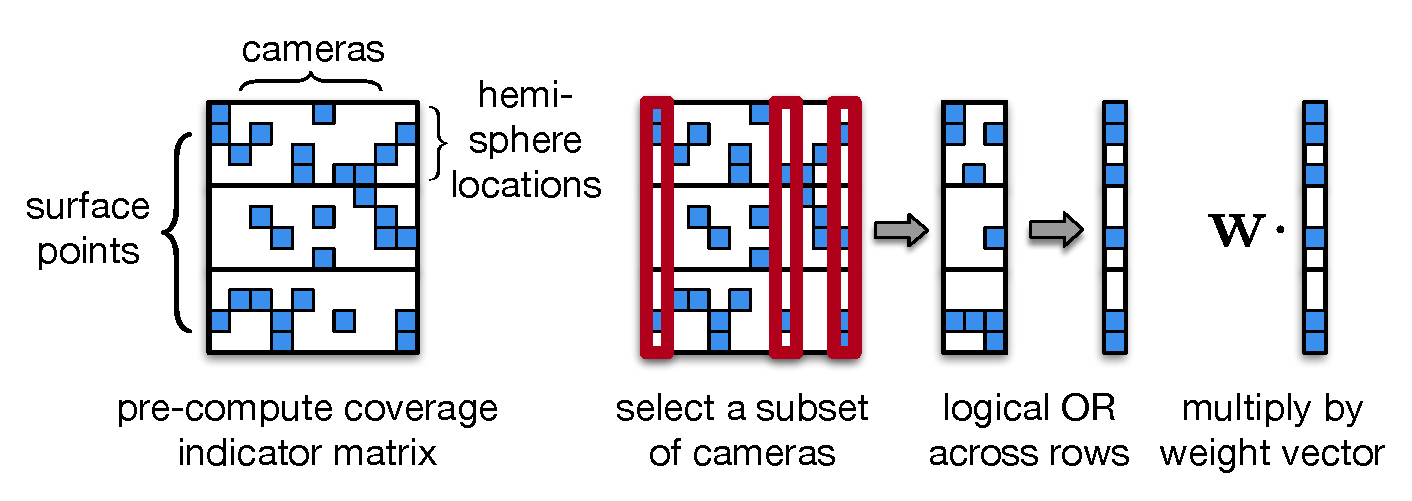
\includegraphics[width=0.47\textwidth]{images/2017_iccv_supplementary/coverage_matrix.pdf}{\vspace{-7pt}}
\end{center}
\caption{
Our matrix representation for efficiently evaluating coverage, for arbitrary subsets of cameras.
We begin by pre-computing a coverage indicator matrix that represents the independent contribution of each camera to the total coverage.
We recover the coverage indicator vector  for a particular subset of cameras by selecting the appropriate subset of columns from our matrix, and performing a logical \textsc{or} operation across the rows of the resulting matrix.
We evaluate our coverage model for this subset of cameras by multiplying the coverage indicator vector with a weight vector.
We use this efficient matrix representation to evaluate coverage for many different subsets of cameras, in our algorithm for generating scanning trajectories.
\vspace{-5pt}
}
\label{fig:coverage_matrix}
\end{figure}

\vspace{-12pt}
\paragraph{Evaluating Coverage for any Subset of Cameras}
In the previous subsection, we showed how to evaluate our coverage model efficiently for a particular set of cameras.
In order to optimize our model, we will need to efficiently evaluate coverage for many different subsets of cameras.
In other words, we would like to efficiently evaluate the following expression, 
%
\begin{equation}
\begin{aligned}
F(C_S) = \mathbf{w}^T \mathbf{v}_S
\end{aligned}
\end{equation}
%
where $C_S \subseteq C$ is an arbitrary subset of cameras;
and $\mathbf{v}_S$ is the coverage indicator vector for the cameras in $C_S$. 

We can efficiently evaluate our model for any subset of cameras $C_S \subseteq C$ by pre-computing a \emph{coverage indicator matrix}, $\mathbf{D}$ (see Figure \ref{fig:coverage_matrix}).
Intuitively speaking, we define the matrix $\mathbf{D}$ to represent the independent contribution of each camera to the total coverage.
Each row of $\mathbf{D}$ corresponds to a particular sampling location on a particular hemisphere.
Each column of $\mathbf{D}$ corresponds to a particular camera in $C$.
Stating our definition of $\mathbf{D}$ more precisely, we set the entry of $\mathbf{D}$ corresponding to \textbraceleft hemisphere $H_j$, hemisphere location $\mathbf{h}_k$, camera $\mathbf{c}_i$\textbraceright ~equal to 1 if \textbraceleft hemisphere $H_j$, hemisphere location $\mathbf{h}_k$\textbraceright ~is covered by the disk $D^j_i$, and equal to 0 otherwise.


\vspace{-5pt}
\section{Designing the Parameters of Our Coverage Model}
\label{sec:evaluating_coverage}

In this section, we provide the exact parameters we use in our coverage model.
In our implementation, we set the radius of each disk $D^j_i$ to decay exponentially as a camera moves away from a surface point.
We chose an exponential decay model as a matter of convenience, because it was intuitive for us to specify disk size in terms of a decay half-life.
When a surface point is not visible from a camera, we define the corresponding disk to have zero radius.
We determine visibility by raycasting against our coarse triangle mesh estimate of the scene geometry.

Stating our model more precisely, we define each disk as the intersection of a hollow unit sphere, centered at the surface point; and a solid cone that has its apex at the surface point, and is oriented towards the camera.
We control the solid angle of each disk by controlling the apex angle of this cone.
We define the apex \emph{half angle} $\theta^j_i$ of each cone in radians as follows,
%
\begin{equation}
\begin{aligned}
\theta^j_i = \theta_\text{max} 2^{ \frac{ -\max(t^j_i - t_0, 0) }{ t_{\text{half}} } }
\end{aligned}
\end{equation}
%
where
$\theta_{\text{max}}$ is the largest possible apex half angle in radians;
$t_0$ is the distance in meters from a camera to a surface point, beyond which our half angle doesn't get any larger;
$t_{\text{half}}$ is the decay half-life of the our half angle in meters; and
$t^j_i$ is the distance from camera $\mathbf{c}_i$ to surface point $\mathbf{s}_j$ in meters.
In our implementation, we set $\theta_{\text{max}} = \frac{1}{2} \frac{\pi}{180} 45$ radians, $t_0 = 4$ meters, and $t_\text{half} = 12$ meters.

In our implementation, we set each weight function $w_j(\mathbf{h})$ to have a cosine-weighted falloff as follows,  
%
\begin{equation}
\begin{aligned}
w_j(\mathbf{h}) = \cos \alpha_\mathbf{h}
\end{aligned}
\end{equation}
%
where $\alpha_\mathbf{h}$ is the angle formed by the hemisphere pole and the vector from the hemisphere origin to the hemisphere location $\mathbf{h}$.



\begin{Listing}[t]
\caption{
The greedy algorithm for maximizing a monotone submodular function, subject to a cardinality constraint and a mutual exclusion constraint.
Evaluating the $\argmax$ expression on line 4 requires evaluating $f$ once for each element in the set $G$, leading to many function evaluations. 
}
\label{lst:greedy}

\begin{algorithmic}[1]

\small

\REQUIRE { ~~\\ \vspace{-7pt}
\begin{itemize}
\item A ground set of elements $C$. \vspace{-7pt}
\item A monotone submodular function $f(C_{S})$ to be maximized, where $C_S \subseteq C$. \vspace{-7pt}
\item A cardinality constraint $|C_{S}| = N$. \vspace{-7pt}
\item A mutual exclusion constraint $C_{S} \in \mathcal{M}$, that defines which elements in $C$ are incompatible.
\end{itemize}
}

\ENSURE  { ~\\ \vspace{-7pt}
\begin{itemize}
\item A subset $C_{S} \subseteq C$ that maximizes $f$ to within 50\% of global optimality, subject to the cardinality constraint and mutual exclusion constraint. \vspace{-12pt}
\end{itemize}
~}

\STATE { $ S \gets \varnothing $ }
\STATE { $ G \gets C $ }

\FOR { $ i \gets 0 \text{ to } N $ }

    \STATE { $ g^{\star} \gets \argmax_{g \in G} f(S \cup g) - f(S) $ }
    \STATE { $ I         \gets \text{all the elements in } G \text{ that are incompatible with } g^{\star} $ }
    \STATE { $ S         \gets S \cup g^{\star} $ }
    \STATE { $ G         \gets G ~\backslash~ \{ I, g^{\star} \} $ }
    
\ENDFOR

\STATE { $ C_S \gets S $ }

\end{algorithmic}
\end{Listing}



\begin{Listing}[t]
\caption{
The lazy greedy algorithm for maximizing a monotone submodular function, subject to a cardinality constraint and a mutual exclusion constraint.
This algorithm maintains a lazily updated list of marginal rewards, $m_g$.
When a marginal reward in this list is stale (i.e., when $u_g = \text{False}$), the value $m_g$ can be interpreted as an upper bound on the true marginal reward, due to submodularity.
This observation can be used to skip a large number of function evaluations.
The lazy greedy algorithm drastically reduces the number of times $f$ must be evaluated, as compared to the greedy algorithm.
}
\label{lst:lazy_greedy}

\begin{algorithmic}[1]

\small

\REQUIRE { ~~\\ \vspace{-7pt}
\begin{itemize}
\item A ground set of elements $C$. \vspace{-7pt}
\item A monotone submodular function $f(C_S)$ to be maximized, where $C_S \subseteq C$. \vspace{-7pt}
\item A cardinality constraint $|C_S| = N$. \vspace{-7pt}
\item A mutual exclusion constraint $C_S \in \mathcal{M}$, that defines which elements in $C$ are incompatible.
\end{itemize}
}

\ENSURE  { ~\\ \vspace{-7pt}
\begin{itemize}
\item A subset $C_S \subseteq C$ that maximizes $f$ to within 50\% of global optimality, subject to the cardinality constraint and mutual exclusion constraint. \vspace{-12pt}
\end{itemize}
~}

\STATE { $ S \gets \varnothing $ }
\STATE { $ G \gets C $ }

\FORALL { $ g \in G $ }

    \STATE { $ m_g \gets f(S \cup g) - f(S) $ }
    \STATE { $ u_g \gets \text{True} $ }

\ENDFOR

\FOR { $i \gets 0 \text{ to } N$ }

    \STATE { $ g^{\star} \gets \argmax_{g \in G} m_g $ }

    \WHILE { $ \text{not } u_{g^{\star}} $ }

        \STATE { $ m_{g^{\star}} \gets f(S \cup g^{\star}) - f(S)$ }
        \STATE { $ u_{g^{\star}} \gets \text{True}$ }
        \STATE { $ g^{\star}     \gets \argmax_{g \in G} m_g $ }

    \ENDWHILE

    \STATE { $ I \gets \text{all the elements in } G \text{ that are incompatible with } g^{\star} $ }
    \STATE { $ S \gets S \cup g^{\star} $ }
    \STATE { $ G \gets G ~\backslash~ \{ I, g^{\star} \} $ }

    \FORALL { $ g \in G $ }

        \STATE { $ u_g \gets \text{False} $ }
    
    \ENDFOR

\ENDFOR

\STATE { $ C_S \gets S $ }

\end{algorithmic}
\end{Listing}

\vspace{-0pt}
\section{The Greedy Algorithm for Maximizing Submodular Functions}
\label{sec:greedy}

In this section, we provide additional details regarding the greedy algorithm for maximizing submodular functions.
The problem in equation (2) in the main paper can be solved to within 50\% of global optimality with the greedy algorithm in Listing \ref{lst:greedy}.
To see that this is the case, we first make the observation that our coverage model is \emph{monotone} (i.e., selecting more camera poses never reduces our coverage score) \cite{krause:2014}.
We also make the observation that our mutual exclusion constraint is an instance of a more general mathematical object known as a \emph{partition matroid constraint} \cite{krause:2014}.
It is known that maximizing a monotone submodular function, subject to a cardinality constraint and a partition matroid constraint, can be solved to within 50\% of global optimality with the greedy algorithm \cite{krause:2014}.

The greedy algorithm can be expensive to run on large problems, because it must evaluate the submodular function many times (Listing \ref{lst:greedy}, line 4).
Indeed, the greedy algorithm takes several hours to run on the problem instances we consider in this paper. 
Fortunately, we can leverage submodularity to avoid a very large fraction of this computational effort.
The main insight in this approach, is that the marginal reward for adding an element only ever decreases as more elements are added to the greedy solution, due to submodularity.
Therefore, we can maintain a priority queue of marginal rewards, and we can \emph{lazily} update this queue.
When a marginal reward in our queue is stale, it can be interpreted as an upper bound on the true marginal reward. 
This insight can be used to safely skip a large fraction of function evaluations, in an approach known as the \emph{lazy greedy} algorithm \cite{krause:2014}.
We provide pseudocode for the lazy greedy algorithm, including the necessary modifications to handle our mutual exclusion constraint, in Listing \ref{lst:lazy_greedy}.
For the problem instances we consider in this paper, the lazy greedy algorithm reduces computation time by several orders of magnitude.

\vspace{0pt}
\section{Detailed Formulation of Orienteering as an Integer Linear Program}

In this section, we transform the orienteering problem in equation (4) in the main paper, into a standard integer linear program.
In this derivation, we follow the formulation of Letchford et al.~\cite{letchford:2013}.
However, we express the objective and constraints from this formulation in matrix form, which makes the problem easier to express in a high-level modeling language (e.g., CVXPY \cite{cvxpy:2016}).

We begin by replacing each undirected edge in our graph with two directed \emph{arcs}, each with the same cost as the original undirected edge.
We use the term arc to refer to a directed edge in our modified graph.
We define the indicator vector $\mathbf{x}$ to represent whether or not each arc is traversed.
We define the indicator vector $\mathbf{y}$ to represent whether or not each node in our graph is visited.
We define the vector $\mathbf{g}$ to contain the cumulative costs incurred so far, when beginning to traverse each arc.
Finally, we define the constant vector $\mathbf{f}$ to contain the additive reward at each each node, and we define the constant vector $\mathbf{r}$ to contain the instantaneous cost of traversing each arc.

To help coordinate our optimization problem, we also define inbound and outbound \emph{node-arc indicator matrices}, $\mathbf{A}^{\text{in}}$ and $\mathbf{A}^{\text{out}}$ respectively.
The rows of these matrices represent the nodes in our graph, and columns represent the arcs.
We set the entry of $\mathbf{A}^{\text{in}}$ corresponding to \{node $n$, arc $m$\} equal to 1 if arc $m$ is an inbound arc for node $n$, and equal to 0 otherwise. 
We define $\mathbf{A}^{\text{out}}$ similarly, but with respect to the outbound arcs.
We use the notation $\mathbf{A}_{R}$ to refer to the row of $\mathbf{A}$ corresponding to the root node (i.e., the node where our path must start and end), and we use the notation $\mathbf{A}_{R'}$ to refer to all the other rows of $\mathbf{A}$.


With this notation in place, we define our integer linear program as follows,
%
\begin{subequations}
\label{eqn:ilp}
\begin{equation}
\begin{aligned}
\mathbf{x}^{\star}, \mathbf{y}^{\star}, \mathbf{g}^{\star} = \argmax_{ \mathbf{x}, \mathbf{y}, \mathbf{g} } \mathbf{f}^T \mathbf{y}
\end{aligned}
\label{eqn:ilp_a}
\end{equation}
%
\vspace{-5pt}
%
\begin{equation}
\begin{aligned}
\text{subject to} ~~~~~ \mathbf{r}^T \mathbf{x} \leq B
\end{aligned}
\label{eqn:ilp_b}
\end{equation}
%
\vspace{-5pt}
%
\begin{equation}
\begin{aligned}
\mathbf{A}^{\text{out}}_{R}  \mathbf{x} & \geq \mathbf{1}             &     \mathbf{A}^{\text{out}}      \mathbf{x}                                          & = \mathbf{A}^{\text{in}}      \mathbf{x} \\
\mathbf{A}^{\text{out}}_{R'} \mathbf{x} & \geq \mathbf{y}_{R'} ~~~~~~ &     \mathbf{A}^{\text{out}}_{R'} \mathbf{g} - \mathbf{A}^{\text{in}}_{R'} \mathbf{g} & = \mathbf{A}^{\text{in}}_{R'} \mathbf{T} \mathbf{x} \\
\end{aligned}
\label{eqn:ilp_c}
\end{equation}
%
\vspace{-4pt}
%
\begin{equation}
\begin{aligned}
0 \leq \mathbf{g} \leq \mathbf{U} \mathbf{x}\\
\end{aligned}
\label{eqn:ilp_d}
\end{equation}
%
\vspace{-10pt}
%
\begin{equation}
\begin{aligned}
\mathbf{x} \in \{0,1\}^M ~~~~~ \mathbf{y} \in \{0,1\}^N ~~~~~ \mathbf{g} \in \mathbf{R}_{+}^M
\end{aligned}
\label{eqn:ilp_e}
\end{equation}
\end{subequations}
%
where
the matrix $\mathbf{T} = \mathbf{diag}( \mathbf{r} )$ helps us to calculate an intermediate matrix of instantaneous costs for inbound arcs;
the matrix $\mathbf{U} = \mathbf{diag}( \mathbf{1}B - \mathbf{r} )$ helps us to define the upper bounds for our cumulative cost variable $\mathbf{g}$;
and $M$ is the number of arcs in our graph and $N$ is the number of nodes. 
In this formulation, $\mathbf{x}$, $\mathbf{y}$, and $\mathbf{g}$ are decision variables, everything else is problem data.
Letchford et al.~refer to this integer linear program as a \emph{single-commodity flow} formulation for the orienteering problem \cite{letchford:2013}.

The objective in this optimization problem (\ref{eqn:ilp_a}) attempts to maximize the reward we collect, by activating as many nodes as possible.
The constraint in (\ref{eqn:ilp_b}) enforces our maximum budget on total path length.
The constraints in (\ref{eqn:ilp_c}) specify that: at least one of the outbound arcs for the root node must be active; the number of active outbound arcs must match the number of active inbound arcs at each node; if an outbound arc is active, then the node at its tail must be active; and the difference in cumulative cost at an outbound arc and a corresponding inbound arc, must match the instantaneous cost of the inbound arc.
The constraint in (\ref{eqn:ilp_d}) enforces that the cumulative costs incurred so far are less than the total budget.
Finally, the constraints in (\ref{eqn:ilp_e}) specify that $\mathbf{x}$ and $\mathbf{y}$ are Boolean indicator vectors, and that $\mathbf{g}$ is non-negative and real-valued.

The problem in equation (\ref{eqn:ilp}) is expressed in a standard form that can be given directly to an off-the-shelf solver.
Given a solution to the problem in equation (\ref{eqn:ilp}), we recover the sequence of visited nodes by following outbound arcs from the root until there are no more nodes to visit.
For each visited node, we look up its corresponding camera pose in our coarsened ground set to obtain a sequence of camera poses.

\vspace{-2pt}
\section{Evaluation Details}

In this section, we provide additional real-world reconstruction results, as well as additional methodological details for our synthetic scene experiments.

\vspace{-12pt}
\paragraph{Real-World Reconstruction Results}
We provide high-resolution renderings of our real-world reconstructions in Figure \ref{fig:results_supplementary}.

\vspace{-12pt}
\paragraph{Methodological Details for our Synthetic Scene Experiments}
When acquiring images for each method, we configured UnrealCV \cite{qiu:2016} to produce RGB images at a resolution of 512$\times$512.

When generating high-resolution reconstructions, we set the \emph{scale} parameter of MVE \cite{fuhrmann:2015} to 0.
We set the \emph{depth} parameter of the Screened Poisson Surface Reconstruction algorithm \cite{kazhdan:2013} to 9, which produces a detailed triangle mesh without overfitting to high-frequency noise in the point clouds estimated by MVE.
As in our explore phase, we clipped the input point cloud against the bounding box $\mathbf{b}_s$.
As a post-processing step, we applied the \emph{surface trimming} tool implemented in the Screened Poisson Surface Reconstruction codebase with a \emph{trim} parameter of 7, and we used MeshLab \cite{cignoni:2008} to remove isolated triangle mesh connected components with fewer than than 50000 faces.
We used the \emph{Gaussian damping} option when running the surface texturing algorithm of Waechter et al.~\cite{waechter:2014}.

When collecting ground truth data, we configured UnrealCV to produce RGB and depth images at a resolution of 2048$\times$2048.
We generated 256 uniformly distributed views on an inward-looking sphere around our scene using standard numerical techniques \cite{devert:2012}.
We set the center of our sphere to be the center of the bounding box $\mathbf{b}_s$, and we set its diameter to be 1.5$\times$ the maximum dimension of $\mathbf{b}_s$, which in our case was 72 meters.
We took care to manually remove images from our set of ground truth views that were inside objects.

When measuring geometric accuracy and completeness, we subsampled our ground truth point cloud to obtain a uniformly sampled point cloud, using the \emph{spatial subsampling} method implemented in CloudCompare \cite{cloudcompare:2017}.
When performing this subsampling operation, we set the minimum space between points to the 95$^{\text{th}}$ percentile of the distribution of nearest-neighbor distances in the original ground truth point cloud, which in our case was 0.0133 meters (i.e., prior to subsampling, 95\% of nearest-neighbor distances in the original ground truth point cloud were less than 0.0133 meters).
We sampled points on each reconstructed triangle mesh using the \emph{mesh sampling} method implemented in CloudCompare \cite{cloudcompare:2017}, where we set the desired sampling density to be $\frac{1}{0.0133^2} = 5653.2308$ points per square meter.

When measuring per-pixel visual error, we departed slightly from the formulation suggested by Waechter et al.~\cite{waechter:2017}.
Waechter et al.~suggest measuring visual error by computing zero-mean normalized cross-correlation (NCC) over small patches, so as to be robust to low-frequency discrepancies in illumination between the ground truth images and the test images (i.e., the images of a reconstructed 3D model).
In our synthetic scene, illumination is controlled perfectly, so we do not need this additional robustness.
Moreover, we found that NCC did not successfully localize the noticeable texturing artifacts on baseline reconstructed 3D\ models (e.g., the texturing artifacts visible in Figure 5 in the main paper).
For these reasons, we computed per-pixel differences in RGB space, instead of computing NCC.

Because we rendered ground truth views using UnrealCV, we needed to map the reconstructed 3D models into Unreal coordinates before rendering them and comparing them to the ground truth views.
In practice, our procedure for mapping into Unreal coordinates (see Section \ref{sec:free_space}) is accurate to within a few pixels, but is not perfect.
To prevent our visual quality metric from being dominated by very small coordinate system alignment errors, we computed per-pixel differences in the following way.
For each ground truth pixel location $\mathbf{z}$, we computed the difference between the ground truth image at $\mathbf{z}$, and each pixel in a 9$\times$9 patch centered at $\mathbf{z}$ in the test image.
We took the minimum difference over this patch as the per-pixel difference at $\mathbf{z}$.
In our experience, this approach provided a good balance between being robust to small alignment errors, while also effectively localizing noticeable texturing artifacts in the reconstructed 3D models.

\begin{figure*}[t]
\begin{center}
\includegraphics[width=0.99\textwidth]{images/2017_iccv_supplementary/results_supplementary.jpg}
\end{center}
\caption{
Qualitative comparison of the 3D reconstructions produced by overhead, random, and our trajectories for three real-world scenes.
Our reconstructions contain noticeably fewer artifacts than the baseline reconstructions.
In all our experiments, we control for the flight time, battery consumption, number of images, and quality settings used in the 3D reconstruction.
Best viewed digitally at high resolution.
\vspace{-6pt}
}
\label{fig:results_supplementary}
\end{figure*}

